\documentclass[12pt]{article}


\usepackage[dvips,letterpaper,margin=0.75in,bottom=0.5in]{geometry}
\usepackage{cite}
\usepackage{slashed}
\usepackage{graphicx}
\usepackage{amsmath}
\usepackage{braket}
\begin{document}

\title{Introduction to Probability Distribution Functions}
\author{Michael Mulhearn}

\maketitle

\section{The  Binomial Distribution}

The Binomial Distribution is the most general of the distributions we'll consider, but it is a bit cumbersome to use in practice.  The more familiar Poisson and Gaussian distributions are limiting cases of this distribution.  

Suppose you repeat a particular process $n$ times, and each time you have the same probability $\epsilon$ of a particular outcome, which, without losing generality, we'll call ``success".  The probability of having exactly $m$ successes after $n$ trials is simply given by:
\begin{displaymath}
P = \sum_i p_i
\end{displaymath}
where $i$ runs over all specific outcomes with $m$ successes and $p_i$ is the probability of each specific outcome.   However, as these specific outcomes all contain exactly $m$ successes, they share the same probability, namely:
\begin{displaymath}
p_i = \epsilon^m (1 - \epsilon)^{n-m}
\end{displaymath}
and so we are left to consider simply the total number of specific outcomes containing $m$ successes.  

The quantity we need is provided by the binomial theorem from mathematics, which states that:
\begin{equation}
\label{eqn:binomt}
(p+q)^n = \sum_{m=0}^{n} \binom{n}{m} \, p^m \, q^{n-m}
\end{equation}
where the binomial coefficients are defined by
\begin{equation}
\label{eqn:binomc}
\binom{n}{m} = \frac{n!}{m! \, (n-m)!}
\end{equation}
and are also often referred to in other contexts as $n$-choose-$m$.  The binomial coefficient simply tells us how many times we can choose $m$ instances of $p$ instead of $q$, from $n$ factors, and so it is precisely the combinatoric factor that we need.

The probability of obtaining $m$ successes after $n$ trials with probability $\epsilon$ is therefore given by:
\begin{equation}
\label{eqn:binom}
P(m; \, n ,\epsilon) = \binom{n}{m} \, \epsilon^m \, (1 - \epsilon)^{n-m}
\end{equation}
which is called the Binomial Distribution.

\section{Mean and Variance}

Given a probability distribution, the most urgent questions are generally ``what is the mean value we can expect from this distribution?" and ``how close to the mean value are most of the outcomes?"  The first answer localizes the distribution while the second answer describes its width.

To calculate the mean value in answer to the first question, we simply calculate a weighted average:
\begin{equation}
\braket{m} \equiv \bar{m} \equiv \sum_m m \, P(m) 
\end{equation}
For a continuous probability distribution, we would integrate instead:
\begin{equation}
\braket{x} \equiv \bar{x} \equiv \int x \, P(x) \, dx 
\end{equation}
We usually answer the second question in terms of the variance, $\sigma^2$, of the distribution:
\begin{displaymath}
\sigma^2 \equiv \braket{(x-\bar{x})^2}
\end{displaymath}
Other answers have problems, e.g. $\braket{x-\bar{x}}$ can be zero or nearly so, even for wide distributions, as long as it is symmetric.  You could fix this by calculating $\braket{|x-\bar{x}|}$ but this is generally much harder to calculate, and less useful, than the variance.  For instance, it is left as an exercise to show that:
\begin{equation}
\label{eqn:varhw}
\braket{(x-\bar{x})^2} = \braket{x^2} -\bar{x}^2
\end{equation}
using the fact that $\bar{x}$ is simply a number, and so $\braket{\bar{x}} = \bar{x}$.  We often write this result equivalently as:
\begin{equation}
\label{eqn:variance}
\sigma^2 \equiv \braket{(x-\braket{x})^2} = \braket{x^2} - \braket{x}^2
\end{equation}
Which shows explicitly that we need only calculate $\braket{x}$ and $\braket{x^2}$ in order to determine the variance of a distribution.

\section{Mean and Variance of the Binomial Distribution}

The mean value of Binomial Distribution is given by:
\begin{eqnarray*}
\bar{m} &=& \sum_{m=0}^n \; m \, P(m) \\
&=& \sum_{m=0}^n \; m \, \binom{n}{m} \epsilon^m (1-\epsilon)^{n-m} \\
\end{eqnarray*}
which looks rather daunting!  The trick is to use the Binomial Theorem (\ref{eqn:binomt}) and define a function of two independent variables p and q given by:
\begin{displaymath}
f(p,q) = (p+q)^n = \sum_{m=0}^n \binom{n}{m} p^m q^{n-m}
\end{displaymath}
We then calculate:
\begin{displaymath}
\frac{\partial f}{\partial p} = n(p+q)^{n-1} = \sum_{m=0}^n m \binom{n}{m} p^{m-1} q^{n-m} \\
\end{displaymath}
and multiplying by $p$ we have:
\begin{displaymath}
np(p+q)^{n+1} = \sum_{m=0}^n m \binom{n}{m} p^m q^{n-m}
\end{displaymath}
which is true for any $p$ and $q$.  We now substitute the particular values $p=\epsilon$ and $q=1-\epsilon$ and find that:
\begin{displaymath}
n \epsilon = \sum_{m=0}^n m \binom{n}{m} \epsilon^m (1-\epsilon)^{n-m} \equiv \sum_{m=0}^n m P(m) = \bar{m}
\end{displaymath}
So the mean value is given by:
\begin{equation}
\bar{m} = n \epsilon
\end{equation}
or the total number of trials times the probability of success for each trial, a wholly plausible answer.

For the variance, we use a variation of the same trick, this time using the second partial derivative:
\begin{displaymath}
p^2 \cdot \frac{\partial^2 f}{\partial p^2} = n(n-1)p^2(p+q)^{n-2} = \sum_{m=0}^n m (m-1) \binom{n}{m} p^{m} q^{n-m} \\
\end{displaymath}
and again putting $p=\epsilon$ and $q=1-\epsilon$ to find that:
\begin{eqnarray*}
n(n-1)\epsilon^2 &=& \sum_{m=0}^n (m^2 -m) \binom{n}{m} p^{m} q^{n-m} \\[5pt]
&=& \sum_{m=0}^n (m^2 -m) P(m) \\[5pt]
&=& \braket{m^2-m} = \braket{m^2}-\braket{m}
\end{eqnarray*}
and as $\braket{m} = n \epsilon$ we have:
\begin{displaymath}
\braket{m^2} = n(n-1)\epsilon^2 + n \epsilon
\end{displaymath}
And so:
\begin{displaymath}
\sigma^2 = \braket{m^2} - \braket{m}^2 = n(n-1)\epsilon^2 + n \epsilon - n^2\epsilon^2
\end{displaymath}
or simply:
\begin{equation}
\sigma^2 = n \, \epsilon \, (1 - \epsilon)
\end{equation}
Note that if $\epsilon=0$ or $\epsilon=1$, there is only one outcome (all failures or all success) and so the variation is zero.

\section{The Poisson Distribution}

Suppose we have some time interval over which we expect to observe a mean number of events $\lambda$.  The events must be independent of one another:  an event occurring at a particular time cannot effect the time at which the next event occurs.  We divide the time interval over which the $\lambda$ events are expected to occur into into $n$ sub-intervals, each with an equal probability to contain an event.  These intervals will be all the same size if the events are uniformly distributed in time, but if the events are not uniformly distributed, the sub-intervals are simply chosen to ensure the probability is the same in each interval.  Once cast this way, we can interpret this as a binomial distribution, with probability to contain an event, by construction, given by $\epsilon = \lambda / n$:
\begin{eqnarray*}
P(m) &=& \binom{n}{m} \epsilon^m (1-\epsilon)^{n-m} \\[5pt]
  &=& \frac{n!}{m! \, (n-m)!} \; \left( \frac{\lambda}{n} \right)^m \left( 1 - \frac{\lambda}{n}\right)^{n-m} \\[5pt]
  &=& \left( \frac{\lambda^m}{m!} \right) \left(1-\frac{\lambda}{n} \right)^n \left[ \frac{n!}{(n-m)!} \cdot \frac{1}{n^m}\right]_1 \left[ \left( 1 - \frac{\lambda}{n}\right)^{-m}\right]_2
\end{eqnarray*}
It is left as an exercise to show that both $[\dots]_1 \to 1$ and $[\dots]_2 \to 1$ as $n \to \infty$.  Recalling that
\begin{displaymath}
\lim_{n \to \infty} \left(1 - \frac{\lambda}{n} \right)^n = e^{-\lambda}
\end{displaymath}
we obtain the Poisson distribution, the probability for observing $m$ events for a mean of $\lambda$:
\begin{equation}
\label{eqn:poisson}
P(m\; ; \; \lambda) = \frac{\lambda^m}{m!} \, e^{-\lambda}
\end{equation}
Notice that there is no longer a parameter $n$, since we took $n \to \infty$, and so $m$ now ranges from 0 to $\infty$.

\section{Mean and Variance of The Poisson Distribution}

The mean of the Poisson distribution is given by:
\begin{eqnarray*}
\bar{m} &=& \sum_{m \geq 0} \; m \, P(m) \\
&=& \sum_{m \geq 0} \; m \, \frac{\lambda^m}{m!} \, e^{-\lambda}\\
\end{eqnarray*}
Since the first term ($m=0$) is zero, we have:
\begin{eqnarray}
\bar{m} &=& e^{-\lambda} \sum_{m \geq 1} \; \frac{\lambda^m}{(m-1)!} \notag \\
             &=& \lambda e^{-\lambda} \sum_{m \geq 1} \; \frac{\lambda^{m-1}}{(m-1)!} \notag \\
             &=& \lambda e^{-\lambda} \sum_{n \geq 0} \; \frac{\lambda^{n}}{n!} \notag \\
             &=& \lambda e^{-\lambda} e^\lambda \notag \\
\bar{m}  &=& \lambda
\end{eqnarray}
which should come as no surprise, as the assumption in the derivation was the that mean number of events was $\lambda$.

For the variance, we use a similar manipulation to calculate:
\begin{eqnarray*}
\braket{m^2} &=& \sum_{m \geq 0} \; m^2 \, P(m) \\
&=& \sum_{m \geq 0} \; m^2 \, \frac{\lambda^m}{m!} \, e^{-\lambda}\\
&=& \lambda \sum_{m \geq 1} \; m \, \frac{\lambda^{m-1}}{(m-1)!} \, e^{-\lambda}\\
&=& \lambda \sum_{n \geq 0} \; (n+1) \, \frac{\lambda^{n}}{(n)!} \, e^{-\lambda}\\
&=& \lambda \braket{m+1} = \lambda \, (\lambda+1)
\end{eqnarray*}
And so:
\begin{eqnarray}
\sigma^2 &=& \braket{m^2} - \braket{m}^2 \notag \\
&=& \lambda \, (\lambda+1) - \lambda^2 \notag \\
\sigma^2 &=& \lambda. 
\end{eqnarray}
That is, the variance of a Poisson distribution is simply the mean.

\section{The Gaussian Distribution}

Next, we consider the Poisson Distribution in the limit $\lambda \to \infty$.  In this case, we can apply the Stirling Approximation:
\begin{displaymath}
\lim_{n \to \infty} n! = \sqrt{2 \pi n} \; e^{-n} \; n^n
\end{displaymath}
to the Poisson distribution as follows:
\begin{eqnarray*}
P(m) &=& \frac{\lambda^m}{m!} \, e^{-\lambda} \\[5pt]
 &\to& \frac{\lambda^m e^{-\lambda}}{\sqrt{2 \pi m} \; e^{-m} \; m^m} \\[5pt]
 &=& \frac{e^{m-\lambda}}{\sqrt{2\pi\lambda}} \left( \frac{\lambda}{m}\right)^{m+\frac{1}{2}}\\
\end{eqnarray*}
Now we consider a new variable $\delta$, defined by
\begin{displaymath}
\delta \equiv \frac{m-\lambda}{\lambda}
\end{displaymath}
which measures the difference between the value $m$ and the mean of the distribution, as a fraction of the mean.  Intuitively, the function is getting very narrow, and so we expect this to be a small quantity, but let's check this.  First we have:
\begin{displaymath}
\braket{\delta} = \frac{\braket{m}- \lambda}{\lambda} = \frac{\lambda - \lambda}{\lambda} = 0
\end{displaymath}
but also:
\begin{displaymath}
\braket{\delta^2} = \frac{\braket{(m-\lambda)^2}}{\lambda^2} = \frac{\lambda}{\lambda^2} = \frac{1}{\lambda}
\end{displaymath}
where we have used the fact that the variance is given by $\braket{(m-\lambda)^2} = \lambda$, and so as $\lambda \to \infty $ we have
\begin{displaymath}
\braket{\delta^2} \to 0
\end{displaymath}
So we can write:
\begin{equation} \label{eqn:mdef}
m = \lambda (1 + \delta)
\end{equation}
where we expect the approximation $\delta \to 0$ to hold as long as we require $\lambda \to \infty$.  So now we can write the distribution in terms of the small quantity $\delta$ and the large quantity $\lambda$ as:
\begin{eqnarray}
\label{eqn:pdelt}
P(\delta) &=& \frac{e^{\lambda\delta}}{\sqrt{2\pi\lambda}} \left( \frac{\lambda}{\lambda (1+\delta)} \right)^{\lambda(1+\delta)+\frac{1}{2}} \notag \\[5pt]
 &=& \frac{e^{\lambda\delta}}{\sqrt{2\pi\lambda}} \cdot \frac{1}{X}
\end{eqnarray}
where we define the quantity:
\begin{displaymath}
X = (1+\delta)^{\lambda(1+\delta)+\frac{1}{2}}
\end{displaymath}
which can be approximated as follows:
\begin{eqnarray*}
\ln X &=& \left( \lambda (1+\delta) + \frac{1}{2} \right) \cdot \ln(1+\delta) \\[5pt]
&=& \left( \lambda (1+\delta) + \frac{1}{2} \right) \cdot \left( \delta - \frac{\delta^2}{2} + \mathcal{O}(\delta^3)\right) \\[5pt]
\frac{\ln X}{\lambda}&=& \left( 1+\delta + \frac{1}{2\lambda} \right) \cdot \left( \delta - \frac{\delta^2}{2} + \mathcal{O}(\delta^3)\right) \\[5pt]
&=& \left( 1+\delta + \mathcal{O}\left(\delta^2\right) \right) \cdot \left( \delta - \frac{\delta^2}{2} + \mathcal{O}(\delta^3)\right) \\[5pt]
&=& \delta + \frac{\delta^2}{2}+ \mathcal{O}(\delta^3),
\end{eqnarray*}
where in the second to last step we used $\mathcal{O}\left(\frac{1}{\lambda}\right) \sim \mathcal{O}\left(\delta^2\right)$.  Neglecting the small quantities, we can approximate
\begin{displaymath}
X = \exp\left( \lambda\delta + \lambda\frac{\delta^2}{2} \right) 
\end{displaymath}
which, when plugged backed into Equation~\ref{eqn:pdelt} yields:
\begin{eqnarray}
\label{eqn:almost}
P(\delta) &=& \frac{e^{\lambda\delta}}{\sqrt{2\pi\lambda}} \cdot \frac{1}{\exp\left( \lambda\delta + \lambda\frac{\delta^2}{2} \right)} \notag \\[5pt]
&=& \frac{1}{\sqrt{2\pi\lambda}} \cdot \exp\left( -\lambda \frac{\delta^2}{2}\right)
\end{eqnarray}
Now notice that Equation~\ref{eqn:mdef} implies that $m$ is quite large, and so may now be treated as a continuous variable, which we will rename $x$ (since $m$ looks like an integer value), hence we have:
\begin{displaymath}
\delta \equiv \frac{m - \lambda}{\lambda} = \frac{x - \lambda}{\lambda}
\end{displaymath}
and likewise we know that the variance of the original Poisson distribution is given by $\sigma^2 = \lambda$, and so we can rewrite Equation~\ref{eqn:almost}
in the (hopefully) more familiar form:
\begin{equation}
\label{eqn:gaussian}
P(x) = \frac{1}{\sqrt{2\pi} \sigma} \cdot \exp\left( - \frac{(x - \lambda)^2}{2 \sigma^2}\right)
\end{equation}
Which is a Gaussian distribution with mean value $\lambda$ and variance $\sigma^2$.  The proof that these quantities are indeed the mean and the variance is left as an exercise.

\section{Histograms and Distributions in Scientific Python}

\begin{figure}[htbp]
\begin{center}
{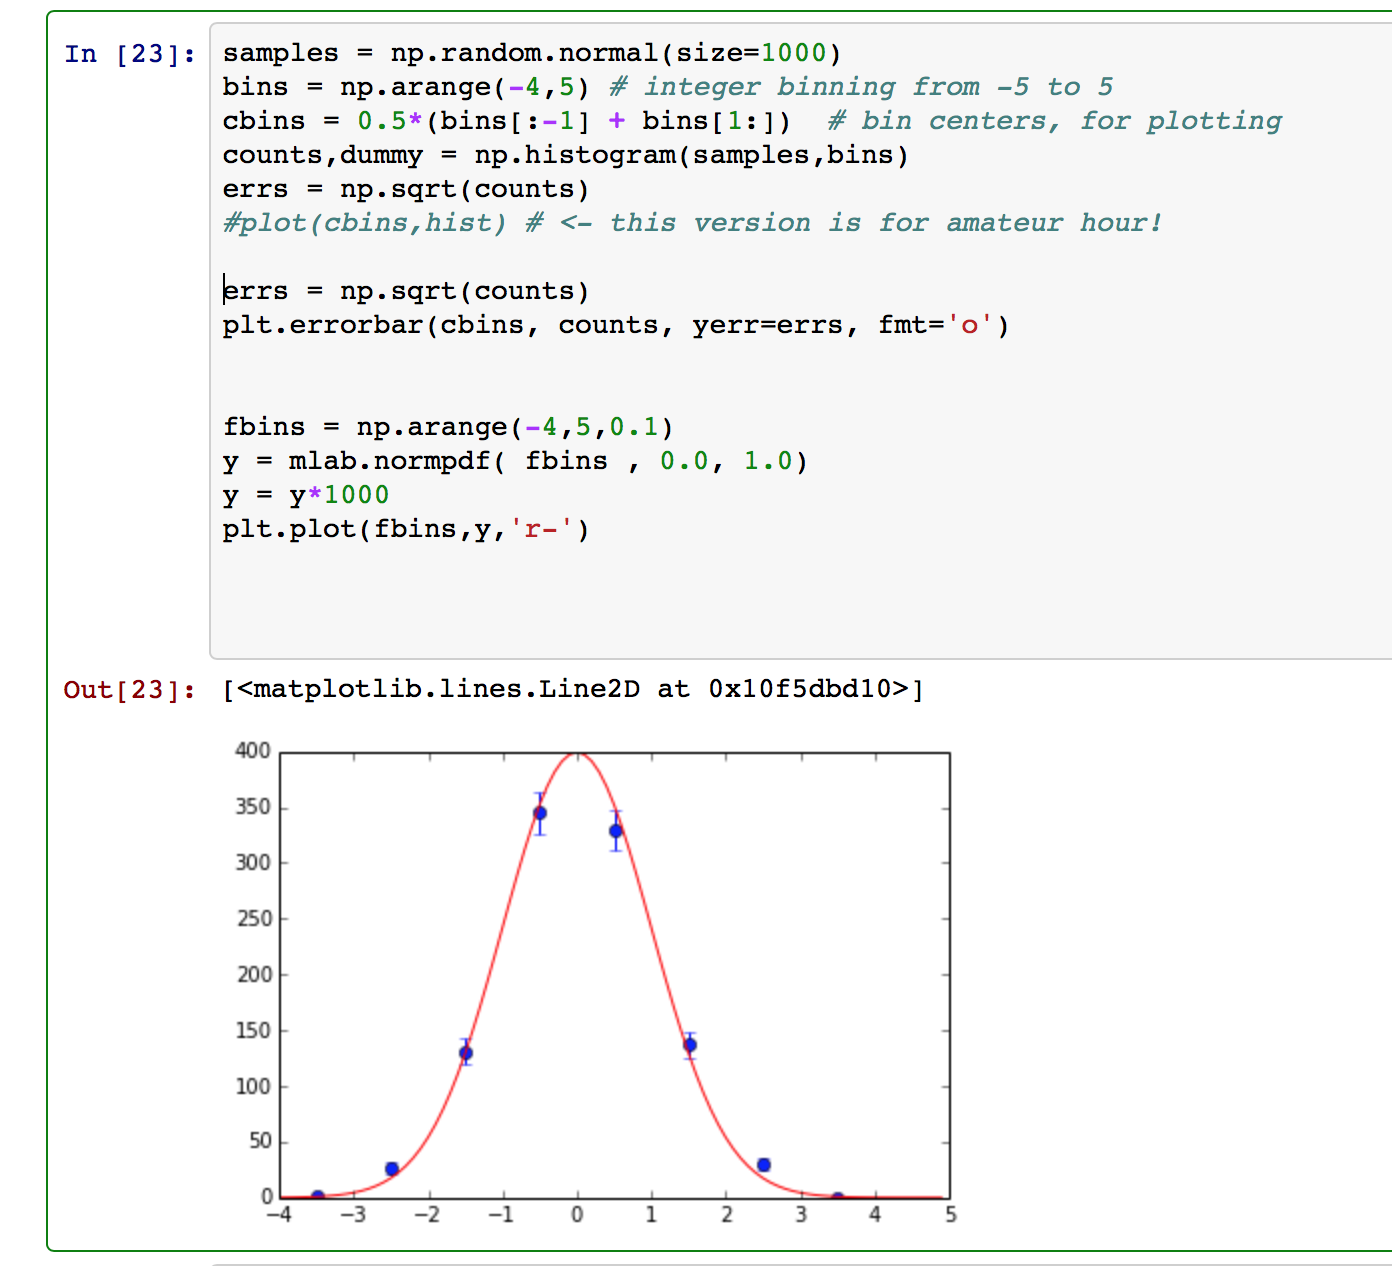
\includegraphics[width=0.95\textwidth]{figs/scipy_hist.png}}
\end{center}
\caption{\label{fig:hist} Histogram.}
\end{figure}

\section{Exercises}

\noindent
{\bf Problem 1:} Show that the Binomial distribution, $P(m)$, in Equation~\ref{eqn:binom} is properly normalized:
\begin{displaymath}
\sum_{m=0}^n P(m) = 1
\end{displaymath}
as a consequence of the Binomial Theorem (Equation~\ref{eqn:binomt}).

\vskip 1cm
\noindent
{\bf Problem 2:} Show that Equation~\ref{eqn:varhw} is correct.

\vskip 1cm
\noindent
{\bf Problem 3:} Show that the Poisson distribution, $P(m)$, in Equation~\ref{eqn:poisson} is properly normalized:
\begin{displaymath}
\sum_{m \geq 0} P(m) = 1.
\end{displaymath}
Hint: recall the Taylor series expansion for $e^\lambda$.

\vskip 1cm
\noindent
{\bf Problem 4:} Show that the Gaussian distribution, $P(x)$, in Equation~\ref{eqn:gaussian} is properly normalized:
\begin{displaymath}
\int_{-\infty}^{\infty} P(x) dx = 1.
\end{displaymath}

\vskip 1cm
\noindent
{\bf Problem 5:} Show that the mean of the Gaussian distribution has been correctly identified in Equation~\ref{eqn:gaussian}.  That is, show explicitly that:
\begin{displaymath}
\int_{-\infty}^{\infty} x P(x) dx = \lambda 
\end{displaymath}

\vskip 1cm
\noindent
{\bf Problem 6:} Show that the variance of the Gaussian distribution has been correctly identified in Equation~\ref{eqn:gaussian}.  That is, show explicitly that:
\begin{displaymath}
\int_{-\infty}^{\infty} x^2 P(x) dx = \sigma^2 
\end{displaymath}
when we take $\lambda=0$ (which is equivalent to simply changing variables $y=x-\lambda$.)
   
%\section{Challenges (Not Assigned)}
%
%\noindent
%{\bf Problem 1:} Prove by induction the formula for the binomial coefficients in (Equation~\ref{eqn:binomc}).
   
\end{document}




